\documentclass[12pt,halfparskip]{scrartcl}

\newcommand{\dokumenttitel}{Erfahrungsberichte}
\usepackage{../bodesuri}


\begin{document}

\title{\dokumenttitel}
\titlehead{
	\centering
	
\includegraphics[width=0.5 \textwidth, clip, trim = 0 7cm 0 0]{design/externes_design/bodesuri_plakat}
	\vspace{2cm}
}
\author{Danilo~Couto, Philippe~Eberli, \\ Pascal~Hobus, Reto~Schüttel, Robin~Stocker}
\maketitle
\newpage

\pagenumbering{roman}

\tableofcontents
\thispagestyle{plain}
\newpage

\pagenumbering{arabic}

\markright{Bodesuri -- \dokumenttitel}


\section{Erfahrungsbericht von Edgar Danilo Couto}

In einem solch grossen Entwicklungs-Projekt war ich bis jetzt noch nicht involviert gewesen. Wie auch schon in anderen Projekten habe ich in diesem wieder viele neue Erfahrungen gesammelt. Die wichtigste Erkenntnis war, wie wichtig die Kommunikation zwischen den einzelnen Projektmitgliedern ist und wie gross der Overhead bei einem grossen Team sein kann. Die Kommunikation zwischen den einzelnen Projektmitgliedern haben wir mittels Sitzungen, E-Mails, Chatclient und IRC sehr gut gemeistert.

Der Anreiz am Projekt war es ein PC-Spiel zu entwickeln mit einem interaktiven GUI. Es war eine neue Herausforderung ein solches GUI zu implementieren und seit einer Ewigkeit auch ein grosser Wunsch meinerseits. Am Anfang sah es danach aus, als ob Swing nicht dafür geschaffen sei und ich hatte es mit Java 2d versucht. Die Möglichkeit von geometrischen Objekten zu gestalten ist in Java 2d hervorragend gelöst. Doch das Ansprechen der einzelnen Objekte im GUI war zu kompliziert. Wir haben uns dann wieder für Swing entschieden. Ich war aber noch sehr skeptisch, aber es erwies sich als eine sehr gute Entscheidung. Der Code sah um einiges einfacher aus und man konnte einfach mittels Observer die Objekte ansprechen und deren neues Aussehen mitteilen. 

Sehr grossen Spass hatte ich auch beim entwerfen der Designs im Photoshop. Ich hatte nicht gedacht, dass es Möglich sei, das komplette Design in Swing zu implementieren, so dass es dem Original Design entspricht. Und mit grossem Erstaunen ist uns auch dies geglückt. Let’s Swing. 

Als neue Technologie im GUI habe ich mich mit XML befasst. Das XML wurde für das Layout verwendet. Jede einzelne Grafik ist mittels Koordinaten auf dem Spielbrett positioniert worden. Das GUI ist so konzipiert, dass man in einem weiteren Schritt ein neues Design entwerfen kann und damit spielen, ohne jeglichen Code umzuschreiben.

Ich habe mich gegen den Schluss auch noch um die Website gekümmert, spricht mit dem Wiki. Ich hatte einige Bedenken, dass man damit eine ansprechende Website erstellen kann. Jetzt sehe ich das völlig anders. Für Dokumentationen jeglicher Art ist das Wiki als Framework die richtige Entscheidung. Das barrierenfreie Design ermöglicht einem durch einfache CSS-Erweiterungen eine anspruchsvolle Website zu entwerfen. In den weiteren Projekten werde ich auf jeden Fall wieder auf das Wiki zurückgreifen.

Als Dokumentation haben wir LaTeX verwendet was für mich ganz neu war. Bis jetzt hatte ich nur Word als Dokumentationswerkzeug verwendet gehabt, welches aber für eine grössere Gruppe nicht geeignet ist. Durch SVN und LaTeX konnten alle Projektmitglieder zur selben Zeit am selben Dokument arbeiten, was sehr gut funktioniert hat. Doch die Möglichkeit der Gestaltung des Dokuments ist beschränkt, was ich persönlich sehr schade finde. In den kommenden Projekten werde ich wieder mit Word die Dokumente erstellen.

Zusammenfassend kann ich dazu sagen, dass das Projekt sehr lehrreich war und trotz der grossen Projektgruppe uns alles sehr gut gelungen ist. Wir hatten eine sehr schöne und amüsante Zeit zusammen, obwohl es mit sehr viel Arbeit verbunden war. Ich möchte mich auf diesem Weg noch bei allen Projektmitgliedern und Helfern für den Einsatz herzlich bedanken.


\section{Erfahrungsbericht von Pascal Hobus}

Als wir ganz am Anfang eine Arbeit suchten, die zu fünft gut umsetzbar und auch noch interessant sein soll, war ich noch etwas skeptisch und wusste nicht so recht was denn nun genau geeignet wäre. Als wir dann auf die Idee kamen das Dog-Spiel auf den Computer zu bringen war das für mich gleich ein grosser Motivationsschub, da ich das Spiel regelmässig mit meinen Freunden zuhause spiele und sehr spannend finde. Nachdem wir das Spiel auch einige Male unter uns gespielt hatten und bei allen die gleiche Motivation erkennbar war machte es auch gleich doppelt Spass, da alle immer an einem Strang zogen.

Am Ende der "<Elaboration"> und zu Beginn der "<Construction 1"> Phase habe ich mich sehr stark um die Architektur des Systems gekümmert. Das Modellieren der Architektur hat mir sehr gefallen, da man schnell auf Schwachstellen und zyklische Abhängikeiten gestossen ist, die man flicken konnte und so die Qualität der Software markant verbessern konnte. Je weiter die Implementierung jedoch voranschritt, desto mehr und desto grössere Refactorings gab es. Es zeigte sich dann, dass man im UML-Tool das Modell mit dem Sourcecode hätte verlinken müssen, damit diese Refactorings erkannt worden wären. Dies war auch ein Grund dafür, warum ich dann nicht mehr in so kurzen Zeitintervallen ein Codereverse durchgeführt habe. Mit der Einführung des Tools Structure 101 hat Reto jedoch eine super Alternative gefunden, um die Package- und Klassenhierarchien zu durchforsten und auf Designfehler zu untersuchen.

Was mich etwas gestört hat war, dass ich nicht immer programmieren konnte. Ich hatte oft Lust jetzt "<endlich"> etwas in Java zu implementieren, musste dann aber feststellen dass schon an allen Baustellen gebaut wurde und es keinen Sinn machte, zu zweit den selben Code zu bearbeiten. Und eine neue Baustelle für ein niedriger priorisiertes Arbeitspaket zu erstellen erschien mir dann auch nicht korrekt. Vor allem in den Phasen "<Construction 2"> und "<Construction 3"> gab es dann aber genug Arbeit um auch interessante Sachen zu implementieren (zum Beispiel Teile des Controllers, die Feldauswahl, das VerbindenView und die Lobby oder die Steuerung der Partnerfiguren).

Mit der Dokumentation in LaTeX hatte ich Anfangs eher mühe. Ich finde das Prinzip einer einfachen Textverarbeitung die mit Subversion verwaltbar ist sehr gut. Wir hatten keine Probleme zu fünft am gleichen Dokument zu schreiben. Sobald ich jedoch meine Gedanken zu Papier bringen wollte, musste ich mich stark mit der Syntax (nur am Anfang) und Formatierungsproblemen auseinandersetzen. Ein WYSIWIG Editor ist für mich an dieser Stelle sehr viel effizienter, da ich mich auf das Wesentliche -- die Dokumentierung -- konzentrieren kann. Für eine Studienarbeit sehe ich LaTeX nicht als geeignetes Instrument, da ich damit einfach zu ineffizient dokumentieren kann. Mein Wunschwerkzeug wäre ein guter WYSIWYG-Editor, der LaTeX generiert.

Die Arbeit mit meinen Kollegen im Team fand ich super. Wir konnten gegenseitige Kritik stets äussern und profitierten meines Erachtens stark von den Stärken der anderen. So bin ich zwar noch nicht zum Konsolen-Freund mutiert, denke aber, dass ich in Zukunft möglichst alle repetitiven Arbeiten zum Beispiel mit einem Ruby-Skript lösen sollte. Was ich persönlich in unserem Projekt super fand, ist die gesamte Infrastruktur und Entwicklerwerkzeuge die wir genutzt haben (Trac, CruiseControl, usw.). Die ganze Thematik der Zeiterfassung war eher ein mühsames Anliegen, da wir einfach kein geeignetes Tool fanden und die Excel-Vorlage auch einige Schwachstellen aufwies.
			
Abschliessend kann ich sagen, dass ich mit dem Projekt sehr zufrieden bin und auch zukünftig noch am Spiel weiterentwickeln möchte. Ich würde vor allem noch gerne die Auswahl der Partnerschaft und einen intelligenten Bot hinzufügen. Ich habe den Eindruck, dass dieses Projekt eine sehr gute Vorbereitung auf die Studienarbeit im kommenden Herbst war.

\section{Erfahrungsbericht von Philippe Eberli}

\section{Erfahrungsbericht von Reto Schüttel}

\section{Erfahrungsbericht von Robin Stocker}

\section{Team-Erfahrungsbericht}

\subsection{Statistiken}
\begin{figure}[h]
	\centering
	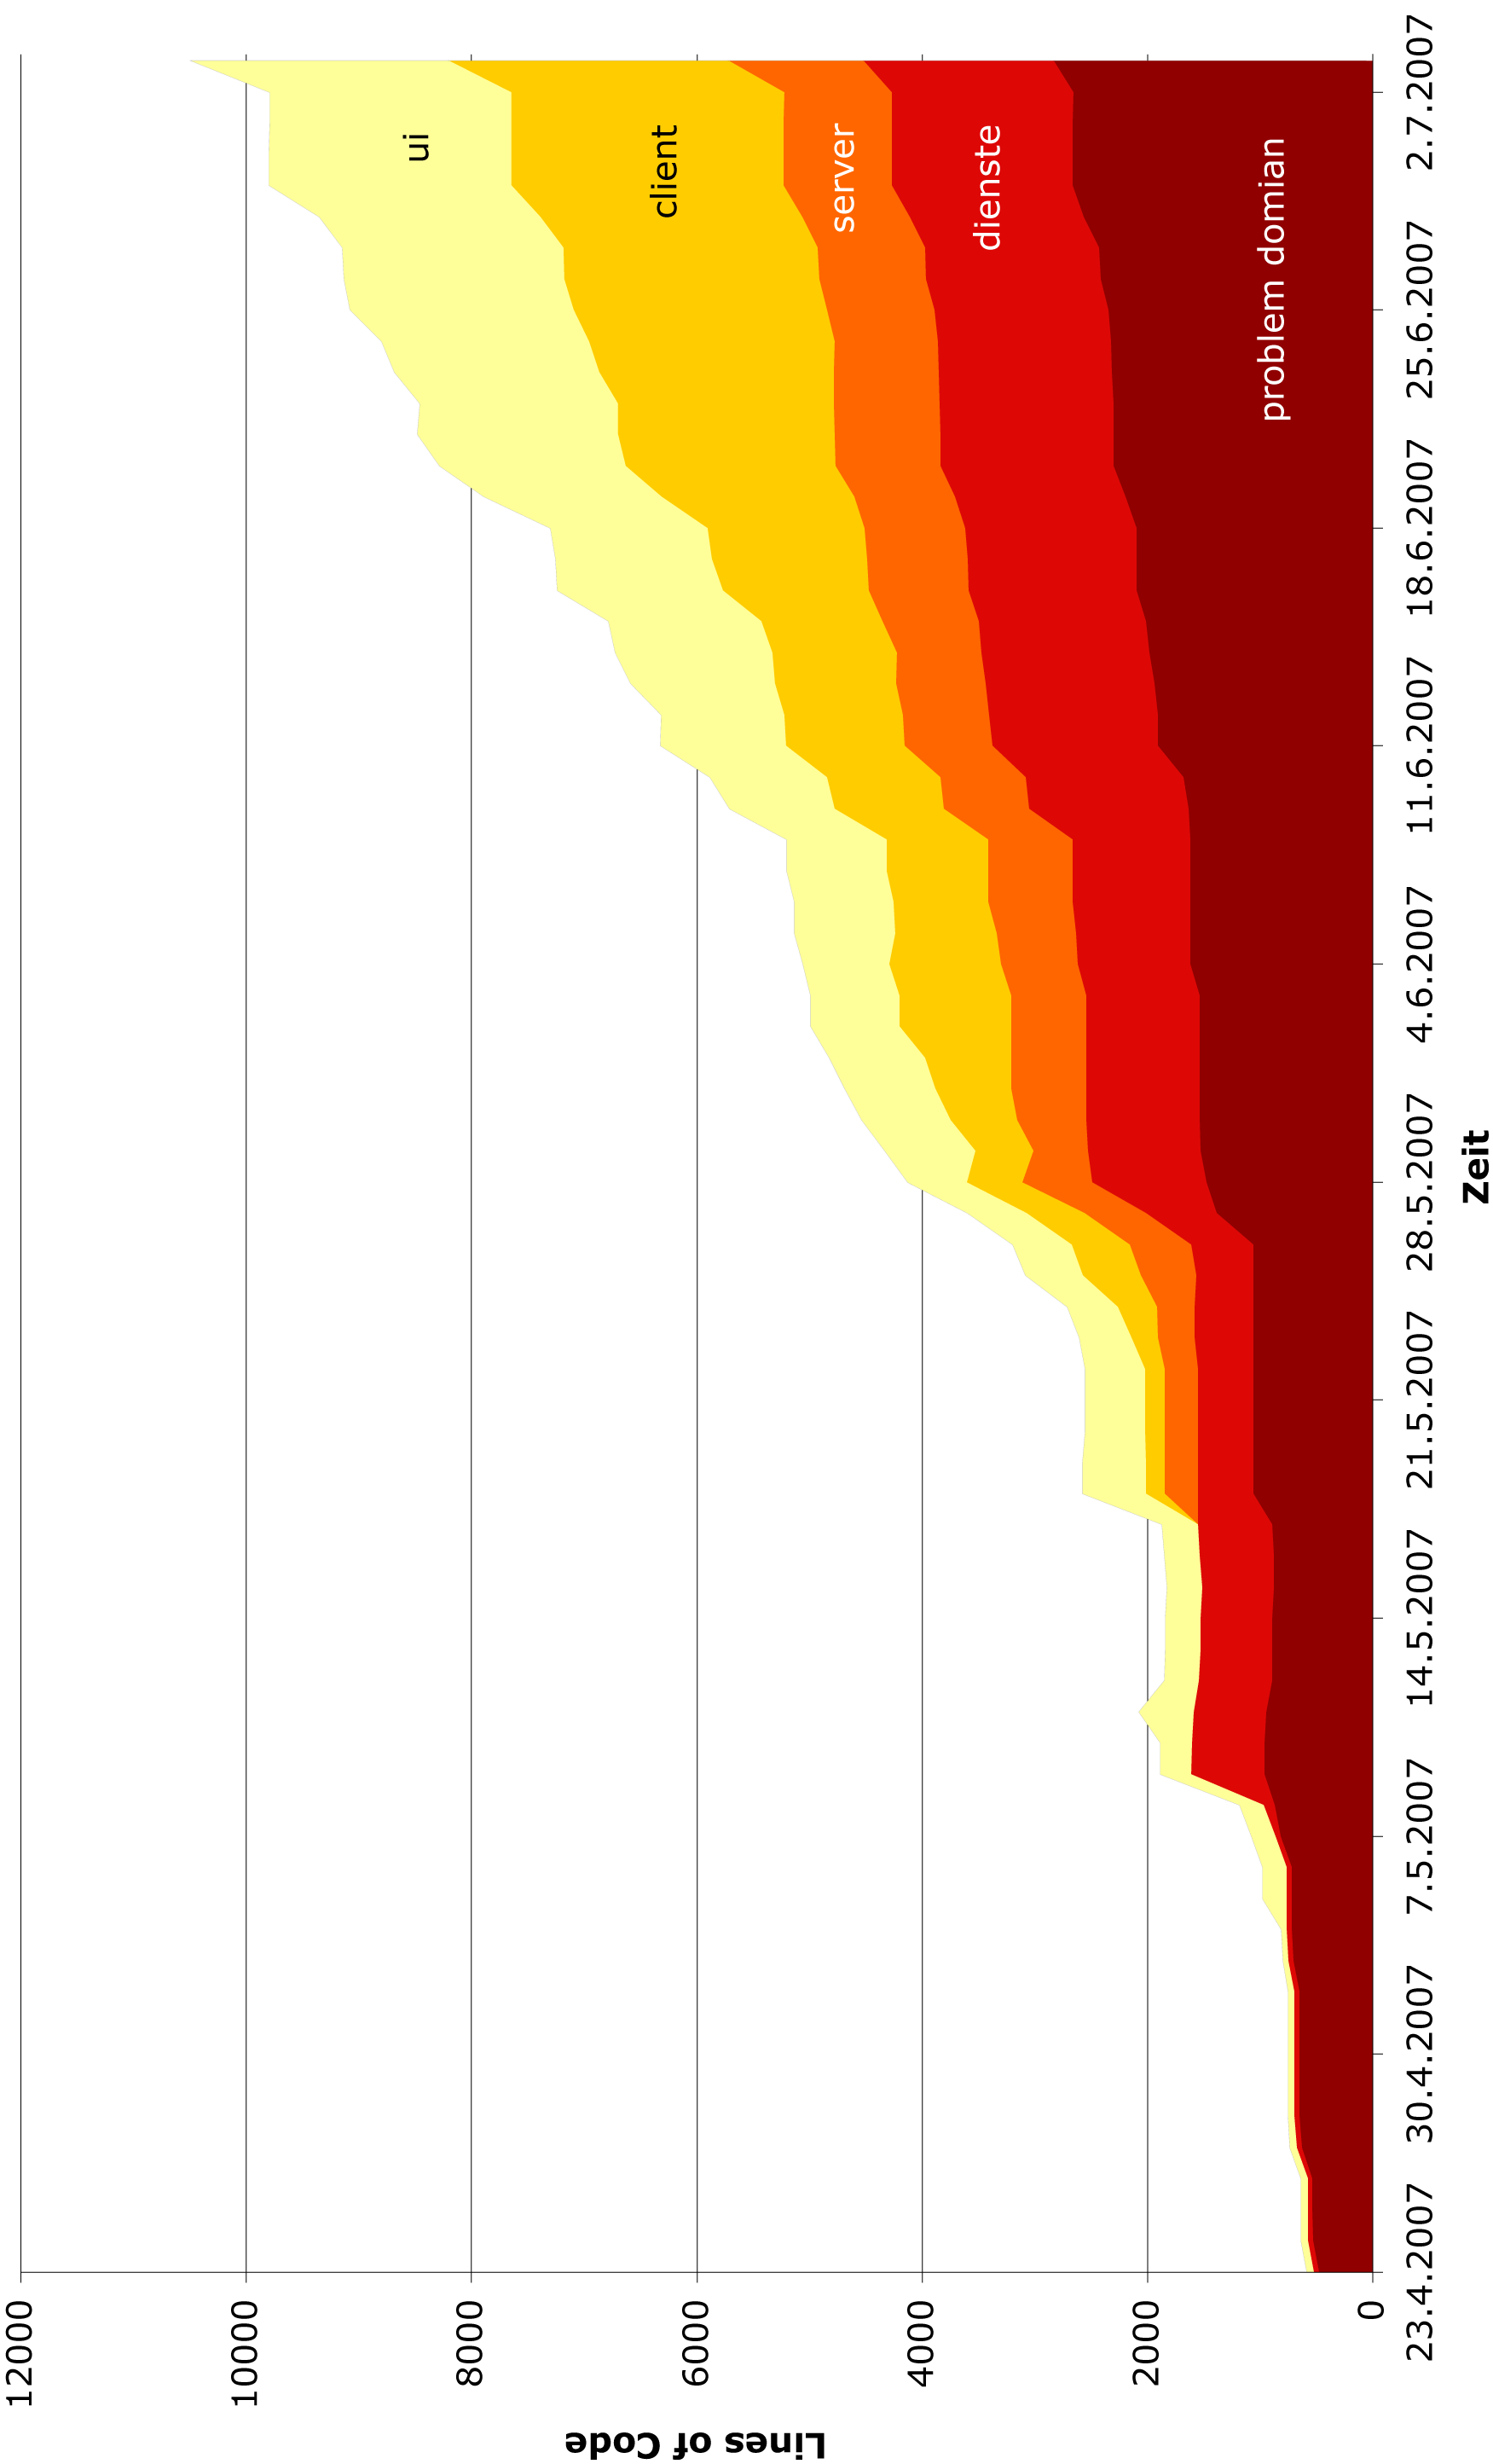
\includegraphics[width=0.8 \textwidth]{anzahl_zeilen_pro_package}
	\caption{Anzahl Zeilen Code pro Package}
	\label{fig:anzahl_zeilen_pro_package}
\end{figure}

\begin{figure}[h]
	\centering
	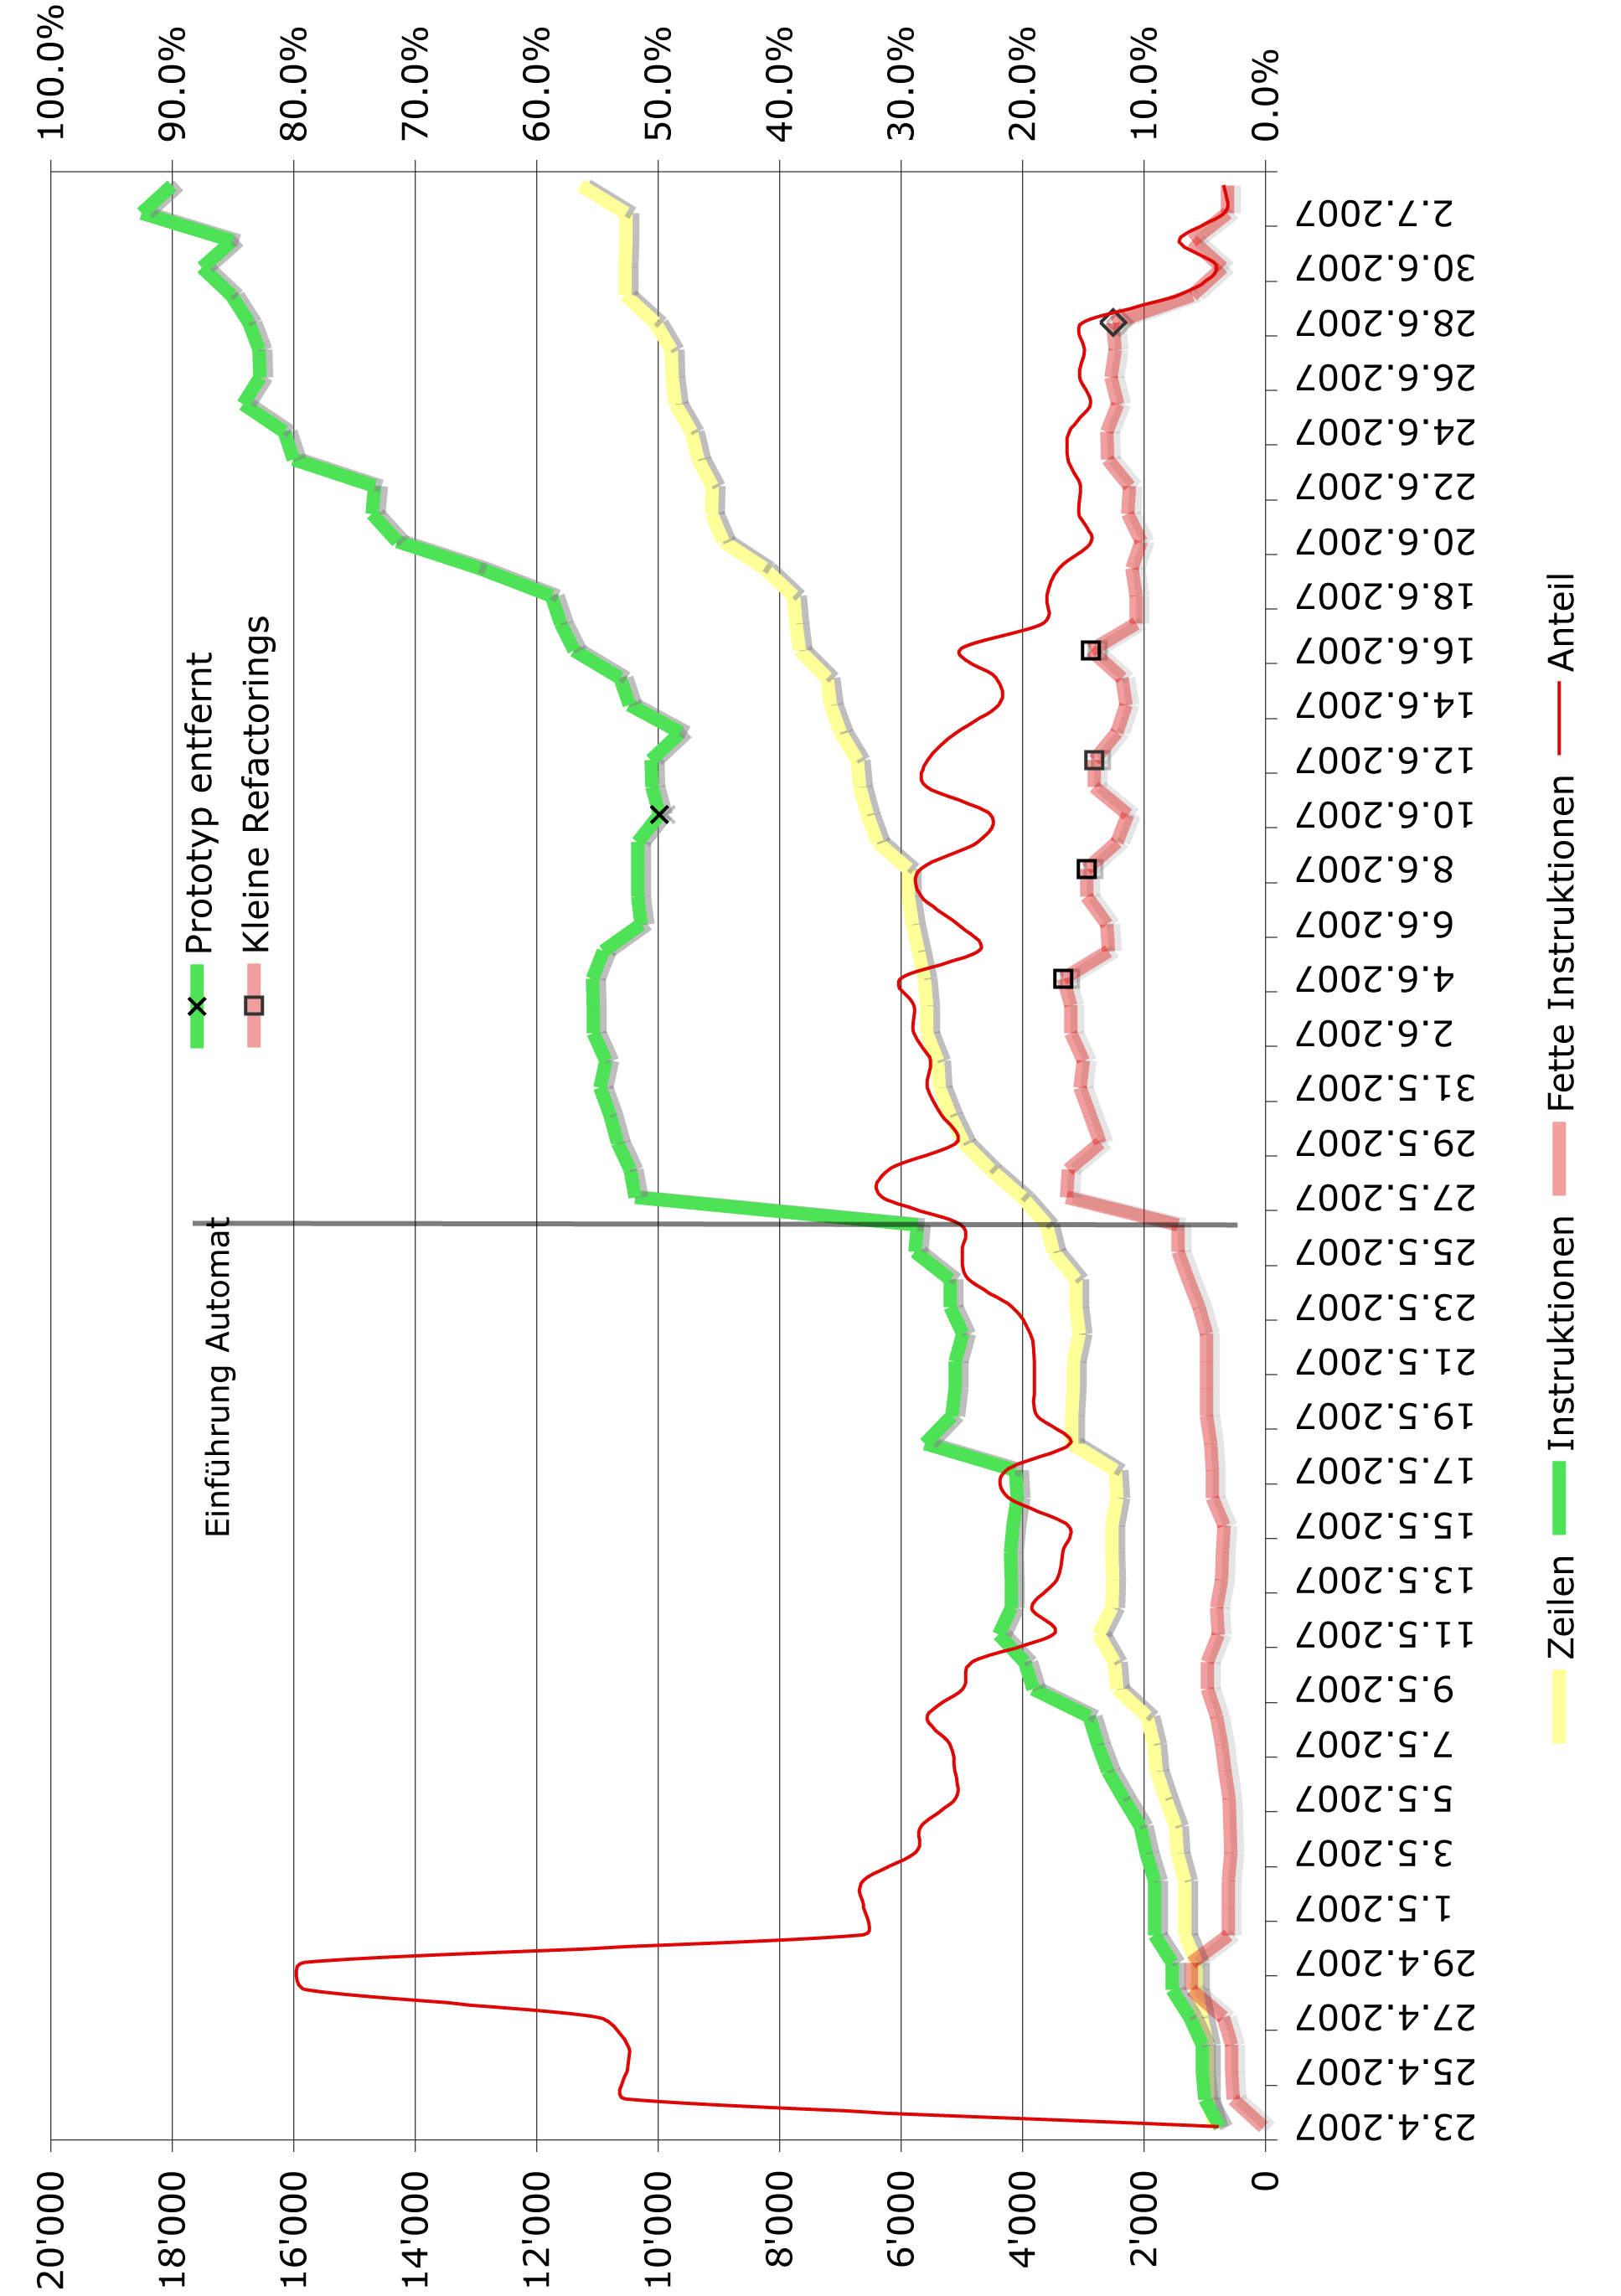
\includegraphics[width=0.8 \textwidth]{code_qualitaet}
	\caption{Aussagen zur Code Qualität}
	\label{fig:code_qualitaet}
\end{figure}

\begin{figure}[h]
	\centering
	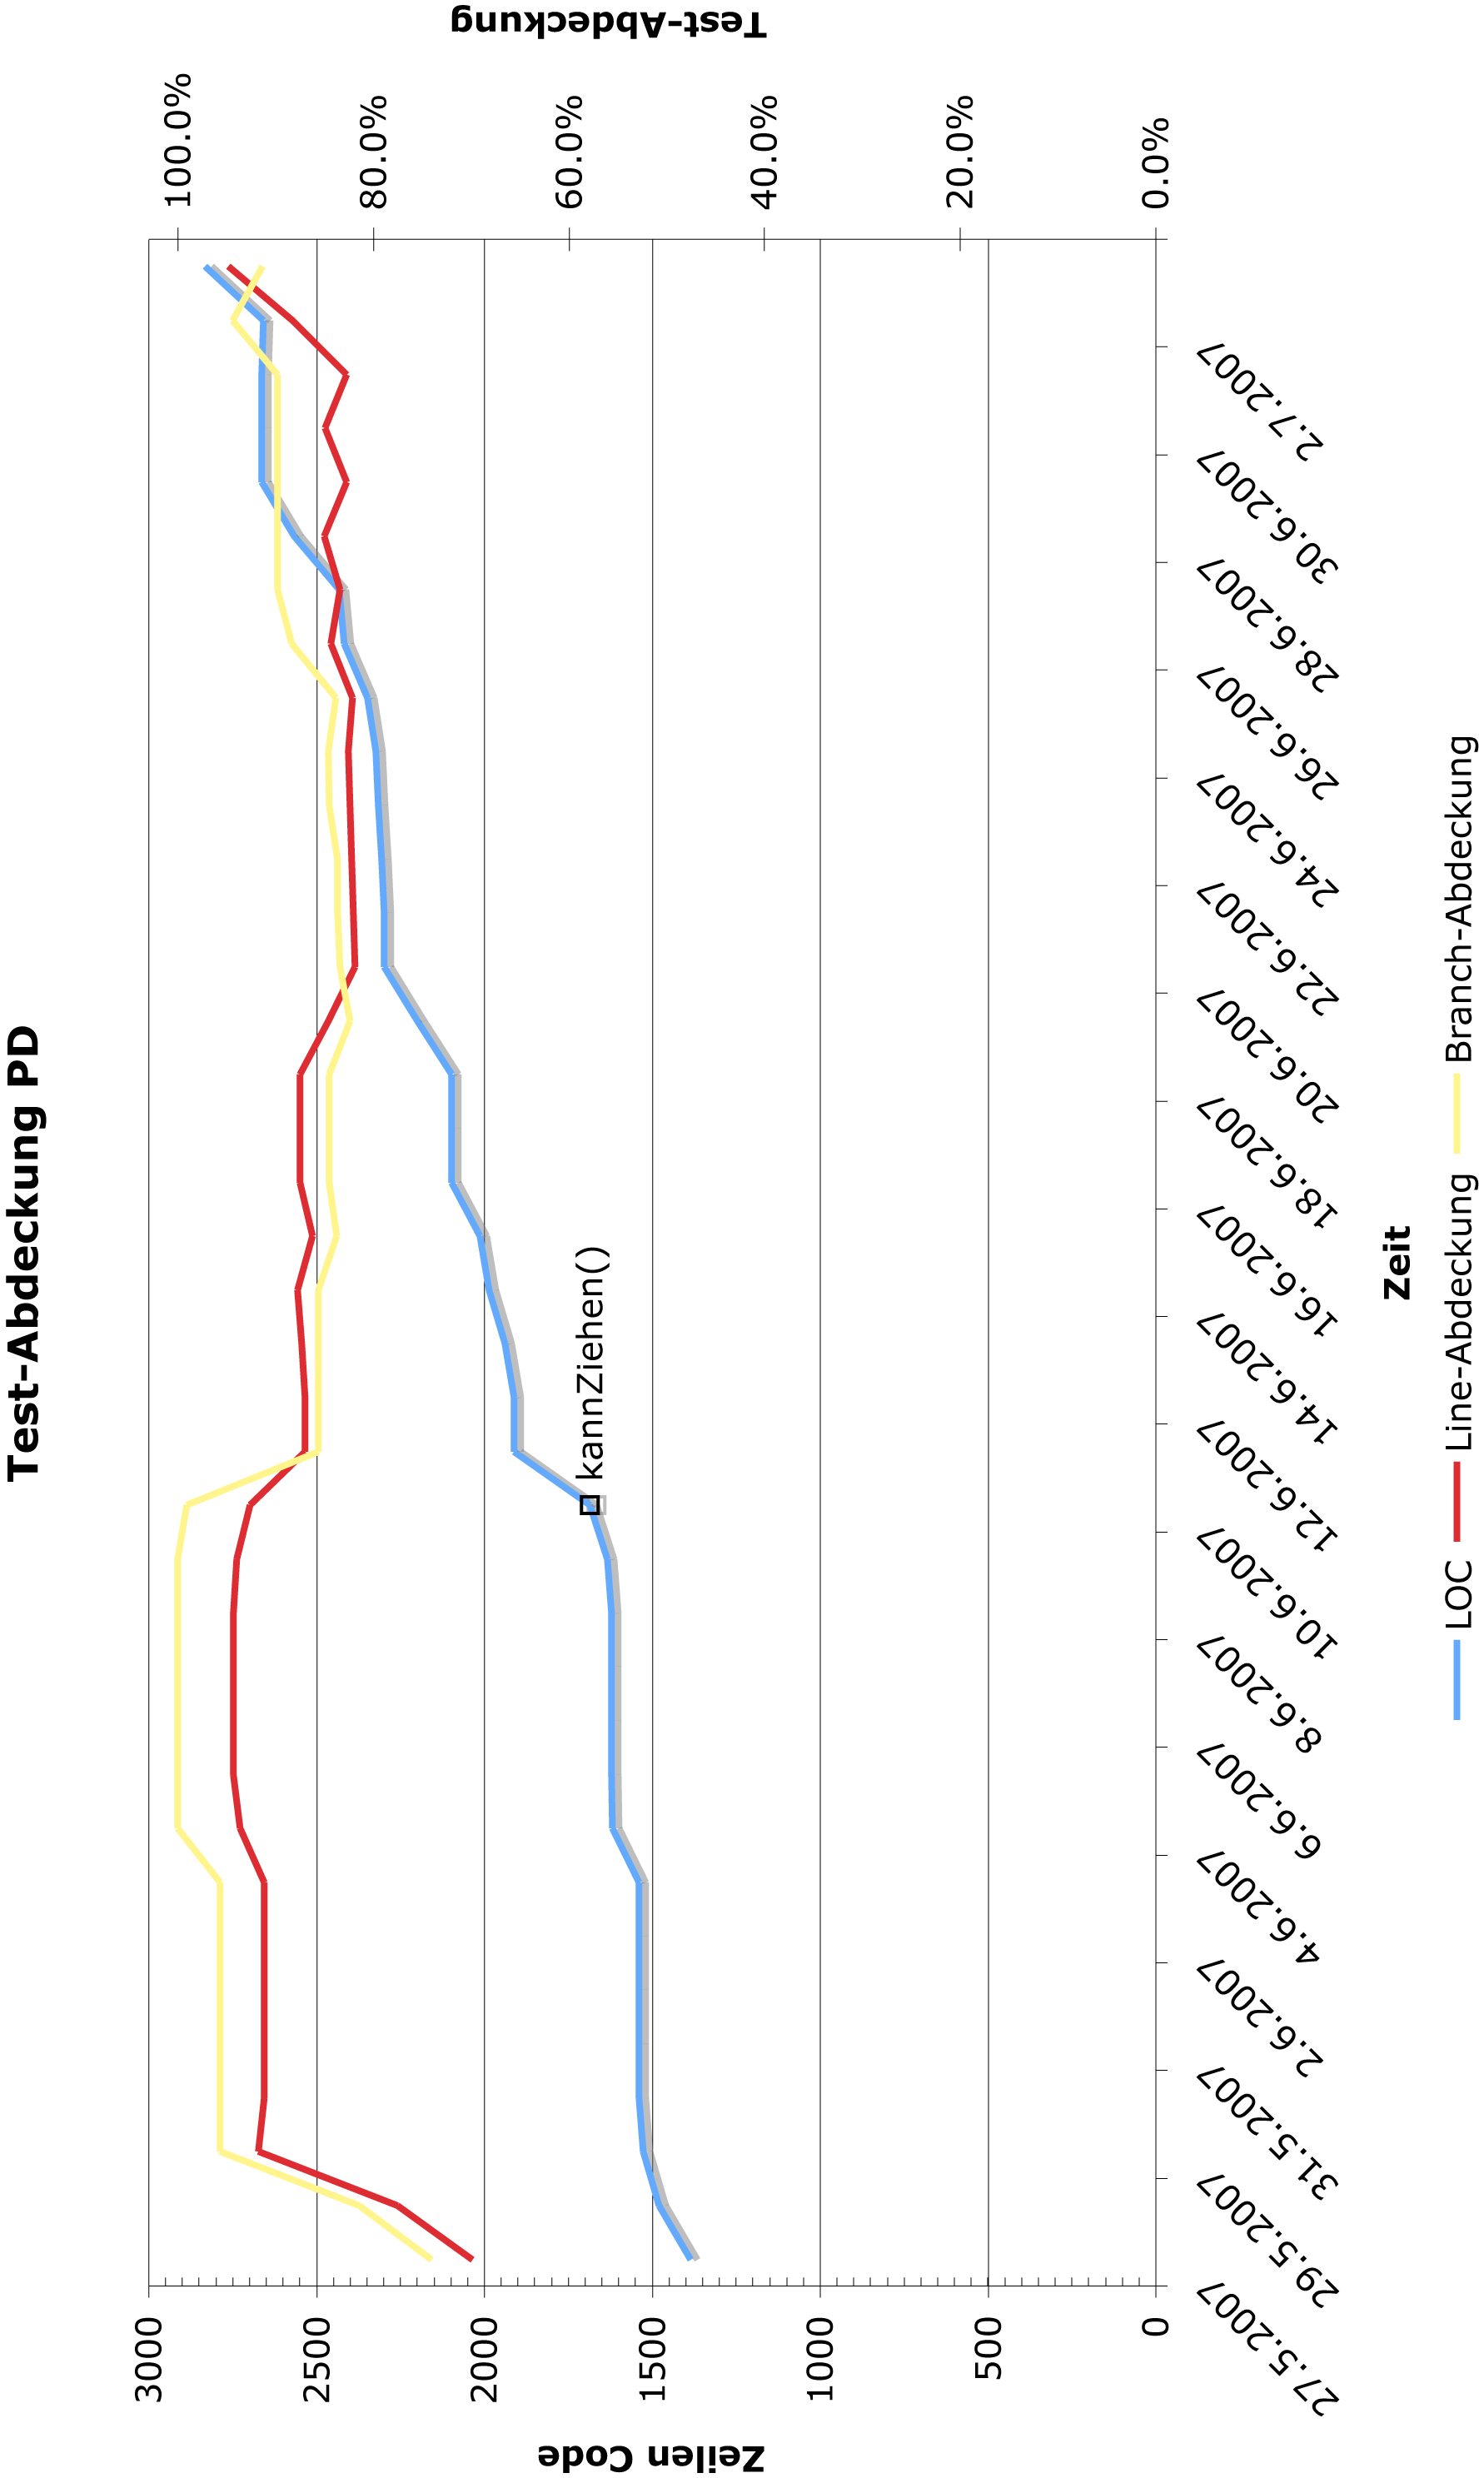
\includegraphics[width=0.8 \textwidth]{test_abdeckung_pd}
	\caption{Testabdeckung der Problem-Domain}
	\label{fig:test_abdeckung_pd}
\end{figure}

\begin{figure}[h]
	\centering
	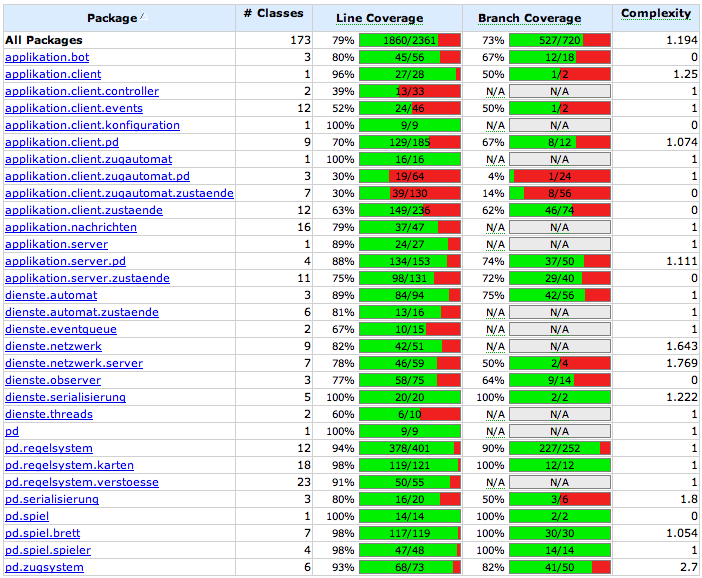
\includegraphics[width=0.8 \textwidth]{test_abdeckung_gesamt}
	\caption{Testabdeckung aller Packages, ausser der UI-Schicht}
	\label{fig:test_abdeckung_gesamt}
\end{figure}

\end{document}
